\documentclass[11pt]{article}
\usepackage[utf8]{inputenc}
\usepackage[myheadings]{fullpage}
\DeclareUnicodeCharacter{0301}{\hspace{-1ex}\'{ }}
% Package for headers
\usepackage{fancyhdr}
\usepackage{lastpage}
\usepackage{titlesec}

% For figures and stuff
\usepackage{graphicx, wrapfig, subcaption, setspace, booktabs}
\usepackage[T1]{fontenc}


% Change for different font sizes and families
\usepackage[font=small, labelfont=bf]{caption}
\usepackage{fourier}
\usepackage[protrusion=true, expansion=true]{microtype}
\usepackage{caption}

\usepackage{multicol}

% Maths
\usepackage{amsmath,amssymb}
\usepackage{float}
\usepackage{graphicx}
\usepackage{wrapfig}
\usepackage[colorinlistoftodos]{todonotes}
\usepackage[colorlinks=true, allcolors=blue]{hyperref}

% Bibliography
\usepackage{biblatex}
\addbibresource{references.bib}

%% Language and font encodings
\usepackage[french]{babel}
\usepackage{csquotes}


\newcommand{\HRule}[1]{\rule{\linewidth}{#1}} % générer une règle horizontale de largeur \linewidth
\onehalfspacing % espacement des lignes à 1,5 fois l'espacement simple
\setcounter{tocdepth}{5} % profondeur table des matières
\setcounter{secnumdepth}{5}

%% Sets page size and margins
\usepackage[a4paper,top=2cm,bottom=1.5cm,left=2cm,right=2cm,marginparwidth=1.5cm]{geometry} %  dimensions de la page et les marges du document

\pagestyle{fancy} % sélectionne le style de page "fancy"
\fancyhf{} % efface les en-têtes et pieds de page actuels

%Header and footer information
\setlength\headheight{15pt} % taille entete 
\fancyhead[L]{Rapport d'analyse} % annotation à gauche de l'entete
\fancyhead[R]{Développement de WebObs} % annotation à droite de l'en-tete
\fancyfoot[R]{\thepage} % afficher le numéro de page à droite du pied de page
\setlength {\marginparwidth }{2cm} % marges latérales de 2 cm


 
\begin{document}

\begin{titlepage}
    \begin{center}
        
    
    % Logo de l'université/entreprise/organisation
    \includegraphics[width=0.2\textwidth]{logo/ensg.png}
    \hspace{2cm}
    \includegraphics[width=0.2\textwidth]{logo/IGN.png}
    \hspace{2cm}
    \includegraphics[width=0.3\textwidth]{logo/ipgp.png}
    \par\vspace{2cm}
    
    % Titre du document
    {\scshape\Huge \textbf{Rapport d'analyse}\par}    
    \vspace{0.5cm}
    {\scshape\Large \textbf{Représentation dynamique de vecteurs de déformation GNSS en 
contexte volcanologique }\par}
    \vspace{1cm}

    \includegraphics[width=0.8\textwidth]{logo/g123.jpg}
    \par\vspace{1cm}

    \begin{multicols}{2}
        % Auteurs
        {\large
        \textbf{Auteurs: }\par
        Clément Monat\par
        Bastien Doré\par
        Nicolas Zito\par
        
        }
        \vspace{1cm}
        
        % Informations sur le client
        {\large
        \textbf{Commanditaires: }\par
        Pierre Sakic, IPGP\par
        François Beauducel, IPGP\par
        }
        \vfill
    \end{multicols}

    \vspace{1cm}
    
    % Autres informations (optionnel)
    {\large Version du Document : 1.0\par}
    
    \vfill
    
    % Bas de page (par exemple, numéro de page)
    {\large \today\par}
    \end{center}
\end{titlepage}


\date{}


\newpage

\tableofcontents
\newpage

\section{Introduction}
Ce projet vise à développer une représentation dynamique des vecteurs de déformation GNSS pour améliorer la surveillance volcanologique effectuée par l'Institut de physique du globe de Paris (IPGP) via WebObs. Actuellement limité à des cartes statiques, WebObs devra intégrer un module interactif avec l'apparition d'une temporalité permettant une visualisation fluide des variations de déformation. 

\section{Contexte du projet}

\subsection{Pour qui?}
   Ce projet est conçu pour répondre aux besoins de l’IPGP et des chercheurs qui utilisent WebObs. 

\subsection{Pourquoi?}
 L’IPGP surveille les quatre volcans actifs du territoire national via ses trois observatoires volcanologiques et sismologiques. Une part essentielle de cette surveillance s’appuie sur des réseaux denses de stations GNSS positionnées sur les volcans, dont le suivi des déplacements constitue un indicateur clé de leur activité. L’ajout d’une dimension temporelle permettrait de mieux visualiser ces mouvements, ouvrant ainsi la voie à des études basées sur des données hebdomadaires.

\subsection{Enjeux}
    L’intégration d’une visualisation dynamique des vecteurs de déformation GNSS dans WebObs présente plusieurs enjeux majeurs :
    \begin{itemize}
    \item Offrir aux volcanologues une compréhension plus fine des phénomènes de déformation en exploitant l’évolution temporelle des données GNSS.
    \item Optimiser l’exploitation des données en facilitant leur interprétation par les chercheurs.
    \item Concevoir une interface intuitive et efficace pour une analyse rapide des tendances et anomalies dans les mouvements de terrain.
    \end{itemize}


\subsection{Aspects financiers et sociaux}
\subsubsection{Coûts du projet}
    Le site web est en open-source, donc gratuit pour l'ensemble des chercheurs à l'IPGP. Les coûts du projet se limitent donc aux coûts de développement : ordinateurs, connexion internet, partage en ligne de fichiers. Tous ces éléments sont fournis gratuitement par l'ENSG ou accessibles chez nous sans impact financier important.
    
\subsubsection{Équipe et répartition des rôles}
    Nicolas Zito, Clément Monat et  Doré Bastien sont développeurs dans le cadre de ce projet.
    En outre, des rôles sont attribués à chacun des membres de l'équipe. Le chef de ce projet, chargé de la communication intra et extra équipe et de la répartition des tâches, est Nicolas Zito. Étant donné les connaissances supplémentaires en interface graphiques, Clément Monat est le responsable du choix de l'interface à implémenter par la suite. Nicolas Zito est responsable de l'architecture du code implémenté et de sa synchronisation via l'outil git avec le code déjà implémenté par les commanditaires. Le test du code et la vérification de la qualité des rendus est attribué à Bastien Doré.



\section{Objectifs de l'étude - Reformulation du besoin}
\subsection{Les objectifs de l'étude}
Objectifs de l'étude :
\vspace{0,1cm}
\begin{itemize}
\vspace{0,1cm}
    \item Créer une visualisation dynamique des données de déformation GNSS :
    \begin{itemize} 
        \item[\textbullet] Avoir un slider pour modifier la fenêtre de données intégrer au calcul de déformations.
        \item[\textbullet] Ajouter un slider permettant de choisir la date à laquelle visualiser les déformations.
    \end{itemize}
    \item Représenter les vecteurs de déformations en 3D sur un modèle SRTM / 3 coupes différentes.
    \item Intégrer la solution au logiciel WebObs déjà existant.
\end{itemize}

\subsection{Les contraintes}
Les contraintes :
\vspace{0,1cm}
\begin{itemize}
\vspace{0,1cm}
    \item La solution implémentée doit utiliser des librairies open-sources.
    \item La solution implémentée peut fonctionner meme si il y a une coupure internet.
    \item Une compatibilité totale avec WebObs, en respectant les contraintes du logiciel et en utilisant des technologies open-source.
   
\end{itemize}


\subsection{Le recueil du besoin - Les acteurs}
Commanditaire :
\vspace{0,1cm}


\begin{itemize}
\vspace{0,1cm}

    \item Besoin d'ajout d'une fonctionnalité sur le site WebObs développé par des chercheurs de François Baudusel chercheur à l'IPGP qui rajoute une temporalité aux cartes pour une étude plus précise des déplacements.
    \item Beoin d'ajout d'une carte en coupe transversale du sol pour mieux visauliser les déformations sur la composante verticale. 
\end{itemize}


\vspace{0,3cm}
Utilisateur Final (chercheurs à l'IPGP) :
\vspace{0,1cm}
\begin{itemize}

    \item Besoin d'un outil intuitif permettant une visualisation dynamique des déformations.
    \item Besoin de modifier la temporalité pour une étude plus précise dans le temps.
    \item Besoin d'une carte en coupe transversale pour mieux visualiser les déformations verticales.
\end{itemize} 

\subsection{Diagramme de cas d'utilisation}
\vspace{0,1cm}
Le diagramme de cas d'utilisation représente les interactions entre les utilisateurs et le système. Il met en évidence les fonctionnalités principales du module de visualisation des vecteurs de déformation GNSS.

Le Chercheur / Ingénieur de l'IPGP peut sélectionner une période d'analyse, manipuler les données de manière interactive et afficher les vecteurs de déformation. Il peut aussi sauvegarder ses préférences d'affichage et exporter les résultats obtenus.

L'Administrateur WebObs est responsable de l'intégration et de l'administration du module dans WebObs.

Les actions de l'utilisateur permettent de mettre à jour l'affichage en temps réel, garantissant une visualisation fluide et dynamique.
\begin{figure}[h!]
    \centering
    \includegraphics[width=15 cm]{use1.png} 
    \caption{Diagramme de cas d'utilisation} 
\end{figure}

\newpage

\section{Analyse fonctionnelle - Solutions proposées}

Afin de répondre aux besoins identifiés, nous avons défini plusieurs fonctionnalités clés permettant d’assurer une représentation dynamique des vecteurs de déformation GNSS sur WebObs. L'objectif principal est de fournir aux chercheurs un outil interactif et intuitif, leur permettant d'explorer plus facilement l'évolution des déformations dans le temps.

Les fonctionnalités majeures proposées incluent :

\begin{itemize}

    \item Un module interactif intégrant des sliders pour ajuster la période d'analyse et sélectionner la date d'affichage des déformations.
    \item Une représentation en 3D des vecteurs de déformation sur un modèle SRTM, avec possibilité d'afficher des coupes transversales pour mieux visualiser la composante verticale.
    \item Le module sera compatible avec l'existant sur WebObs.
    \item Affichage instantané des données grâce à une base préchargée minimisant les requêtes serveur.
    \item Consultation fluide et réactive des données, sans latence liée aux requêtes serveur.
    \item Mise à jour et affichage optimisés des données en temps réel grâce à une gestion avancée du cache.
    
\end{itemize} 


Pour formaliser ces fonctionnalités et proposer une solution adaptée, nous avons élaboré plusieurs diagrammes UML, dont un diagramme de classe détaillant la structure du module, un diagramme de séquence décrivant l'interaction entre les différentes composantes.

Ces diagrammes constituent une première modélisation du projet, qui pourra évoluer en fonction des retours et des ajustements nécessaires lors de l’implémentation.

\subsection{Diagramme de séquence}
\vspace{0,1cm}
Diagramme de séquence :

Ce diagramme décrit le processus permettant à un utilisateur d’afficher des vecteurs de déformation via une interface web interactive. En manipulant un slider, l’utilisateur sélectionne une période, ce qui déclenche une requête au Module Sliders. Celui-ci interroge le Backend WebObs, qui récupère les fichiers de vecteurs et d’erreurs depuis la Base de Données.

Les données filtrées sont ensuite transmises à l’interface web, mettant à jour l’affichage des vecteurs sur une carte topographique 3D SRTM. Ce système optimise les requêtes au serveur en exploitant une base de données préchargée, garantissant une visualisation fluide et interactive.

\begin{figure}[h!]
    \centering 
    \includegraphics[width=0.8\textwidth]{Diagramme_séquence.png} 
    \caption{Diagramme de séquence} 
\end{figure}

\newpage
\subsection{Diagramme de classe}
\vspace{0,1cm}
Diagramme de classe :

Nous créons en amont une base de données contenant tous les fichiers de calculs nécessaires pour limiter les requêtes faites au serveur. Ensuite, les sliders permettent de choisir quels fichiers sélectionner dans cette base de données afin d’obtenir, sur la période choisie et à la date choisie, les vecteurs de déformation avec les ellipses d’erreur. Chaque vecteur est défini par une vélocité dans les trois directions de l’espace, de même pour les ellipses avec les valeurs des erreurs. Ces vecteurs et ellipses sont ensuite représentés dans une carte dont le fond sera un modèle topographique 3D SRTM produit par la NASA et libre.

\begin{figure}[h!]
    \centering 
    \includegraphics[width=0.8\textwidth]{Diagramme_Classe_PDI.jpeg} 
    \caption{Diagramme de classe} 
\end{figure}


\section{Étude technique : Choix des logiciels et langages-Architecture}

 \subsection{Diagramme de déploiement}
\vspace{0,1cm}
Diagramme de déploiement :

Nous pouvons simplifier le fonctionnement de WebObs comme ceci, sachant que nous ne travaillons que sur l’interface dynamique côté client, nous n’interviendrons pas dans la partie serveur de WebObs. La solution que nous devons proposer ne sert qu’à visualiser des données déjà existantes que nous récupérons dès le début sur le serveur de WebObs. Ainsi, notre solution sera directement liée à l’utilisateur.

\begin{figure}[h!]
    \centering 
    \includegraphics[width=0.8\textwidth]{Diagramme_Deploiement_PDI.jpeg} 
    \caption{Diagramme de déploiement} 
\end{figure}

\newpage 
Pour le choix des bibliothèques, chaque membre du groupe a testé différentes solutions pour la représentation dynamique et le fond de carte. Widget est préféré à Bokeh et Dash en raison de sa flexibilité et de sa gestion optimisée des interactions via `ipywidgets` et `traitlets`, qui permettent une synchronisation fluide entre les entrées utilisateur et les calculs en arrière-plan sans nécessiter de serveur intermédiaire, contrairement à Dash qui repose sur Flask et ReactJS, introduisant ainsi une latence supplémentaire. De plus, **Widget** s’intègre naturellement à l'écosystème scientifique Python, notamment avec Matplotlib, NumPy et Pandas, facilitant le traitement et l'affichage interactif des données GNSS en temps réel (cf. [documentation `ipywidgets`](https://ipywidgets.readthedocs.io/en/latest/)).

Concernant le fond de carte, Cartopy est choisi plutôt que Plotly pour sa gestion avancée des projections cartographiques et des données géoréférencées. Contrairement à Plotly, qui est limité au Web Mercator et aux formats GeoJSON, Cartopy prend en charge un large éventail de systèmes de coordonnées via PROJ.4 et Shapely, garantissant ainsi une précision indispensable pour les études de déformation GNSS en contexte volcanologique. De plus, Cartopy permet d’intégrer directement des fonds de carte scientifiques (ex. : MNT, données raster, couches shapefiles), essentiels pour analyser les déformations du terrain (cf. [documentation Cartopy](https://scitools.org.uk/cartopy/docs/latest/)). Son intégration native avec **Matplotlib offre une personnalisation fine des cartes et des annotations, permettant une représentation rigoureuse des vecteurs de déformation GNSS. Ces choix garantissent ainsi des performances optimales et une compatibilité accrue avec les standards géodésiques et volcanologiques.
\section{Réalisation et suivi de projet}

\subsection{Les risques}

\begin{figure}[h!]
    \centering 
    \includegraphics[width=14cm]{risk4.png} 
    \caption{Matrice des risques partie 1} 
\end{figure}

\begin{figure}[h!]
    \centering 
    \includegraphics[width=14cm]{risk3.png} 
    \caption{Matrice des risques partie 2} 
\end{figure}

\newpage


\subsection{Le planning prévisionnel}

Pour ce qui est du planning prévisionnel, on a tout d'abord une partie gestion du fil directeur du projet avec un diagramme de PERT pour savoir si l'on ne dévie pas de l'objectif du projet. Le diagramme de Pert ci-dessous [\ref{pert}] nous présente les différentes tâches à réaliser et leur dépendance. Les flèches en rouge représentent le chemin critique. Les chiffres dans les cases représentent le temps minimal à gauche et maximal à droite pour le début de cette tâche. 

\begin{figure}[h!]
    \centering 
    \includegraphics[width=19cm]{pert1.png} 
    \caption{Diagramme de PERT} 
    \label{pert}
\end{figure}

\newpage

Ensuite, il y a un planning prévisionnel [\ref{plan}] avec les timings pour l'exécution des taches, mais aussi la répartition des taches au sein de l'équipe. Les taches en vert sont les tâches communes.

\begin{figure}[h!]
    \centering 
    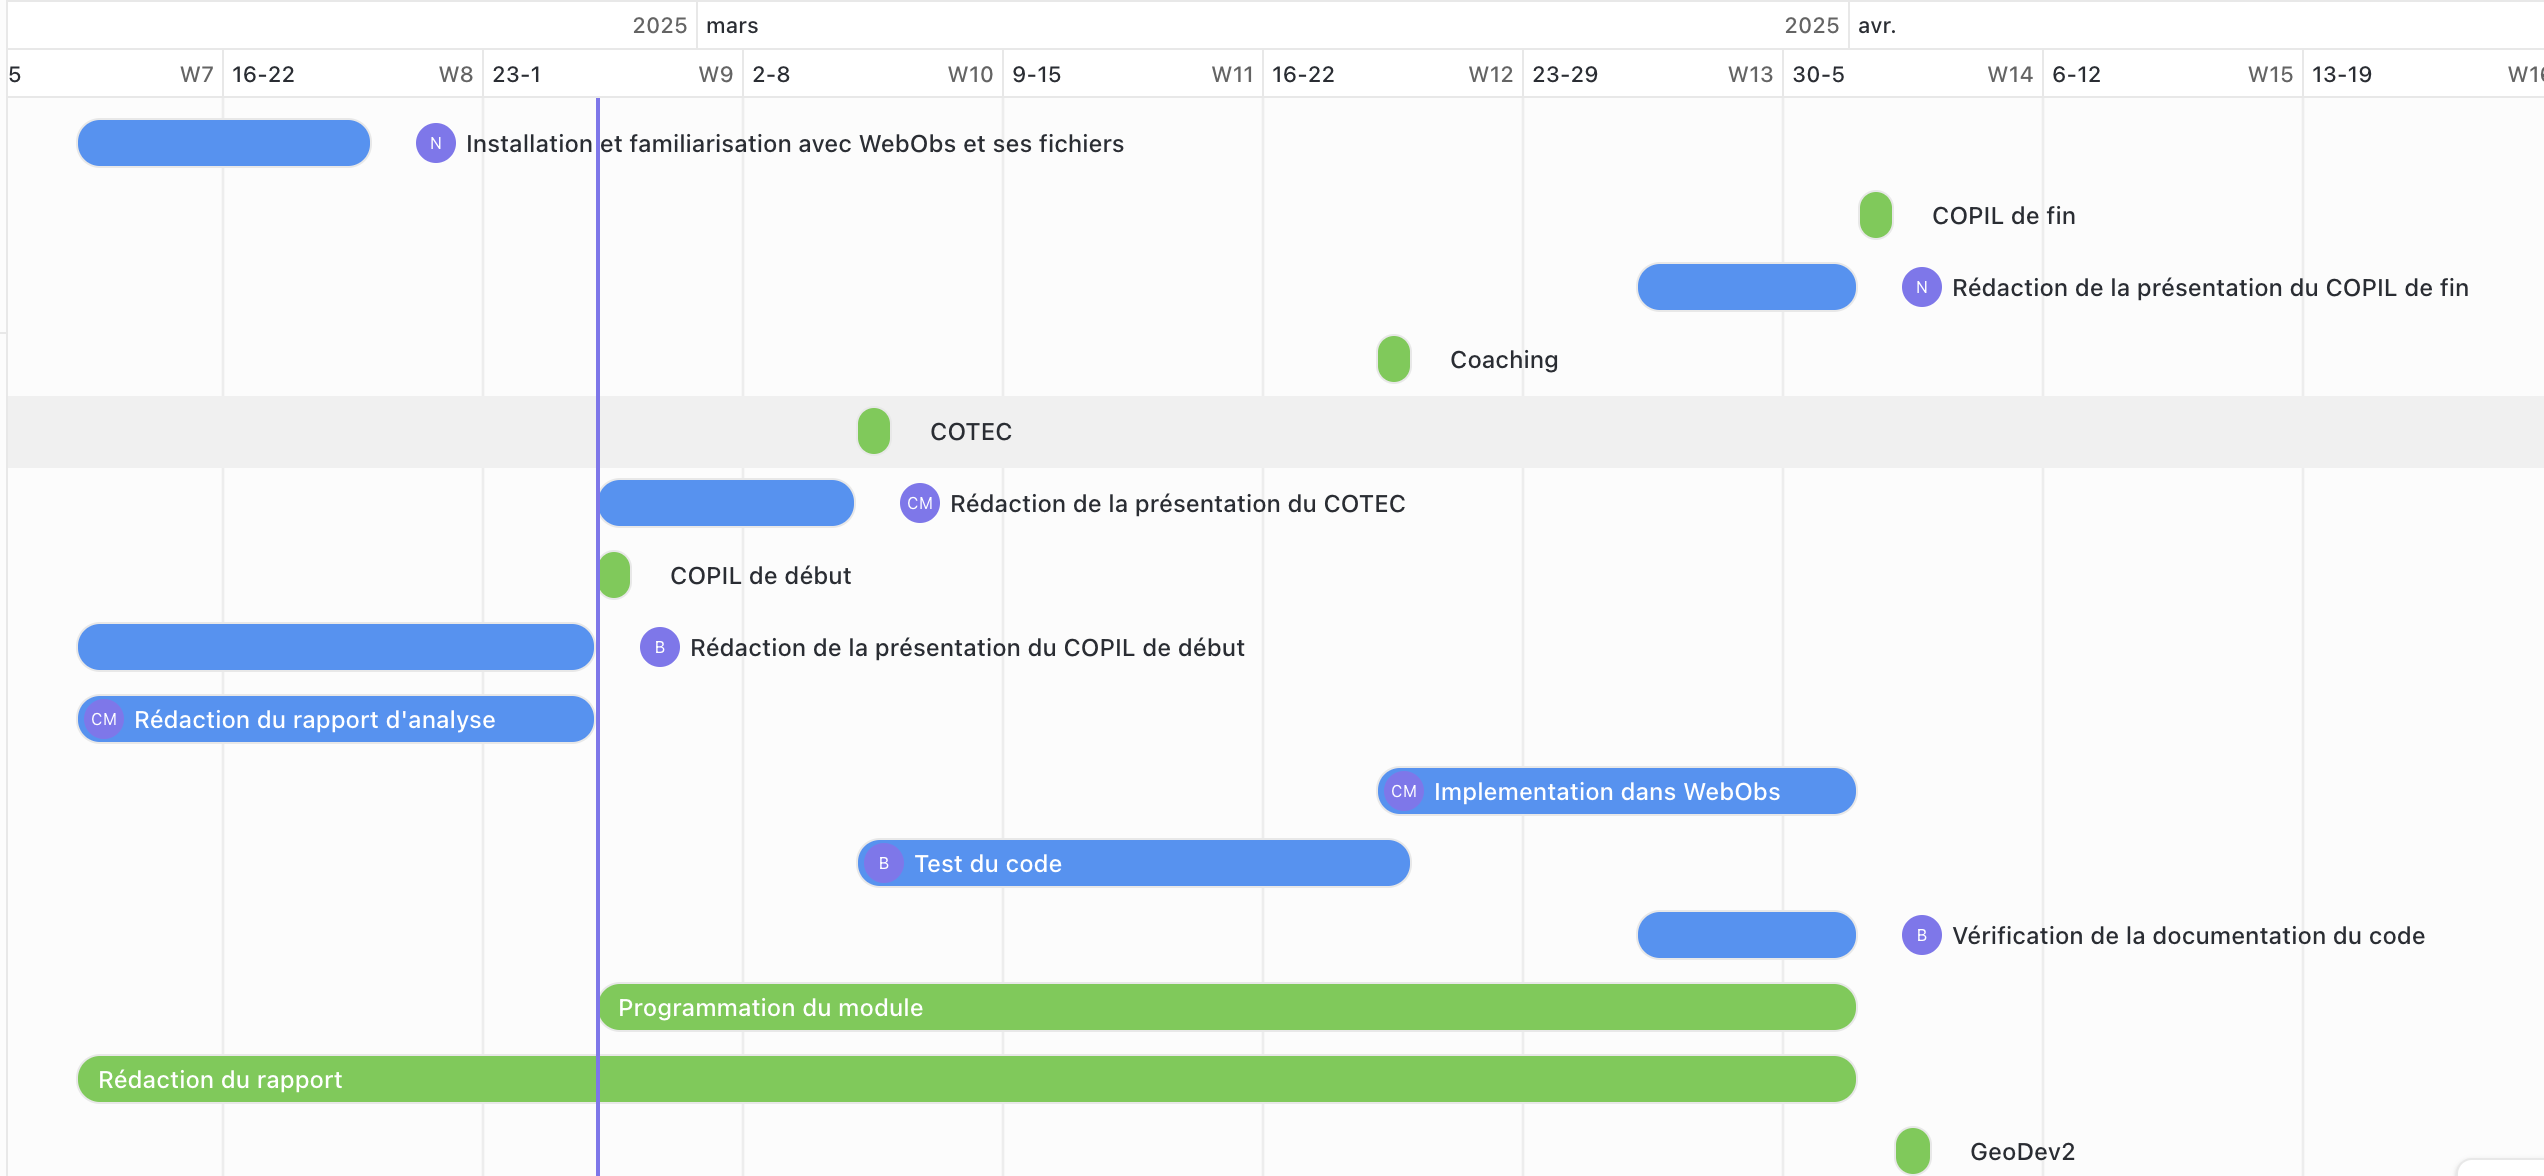
\includegraphics[width=18cm]{Plan.png} 
    \caption{Planning prévisionnel} 
    \label{plan}
\end{figure}

\subsection{Organisation}

Nous avons opté pour l'utilisation de Google Drive pour stocker tous les fichiers pour la gestion du projet comme les captures d'écran des différents diagrammes, tandis que GitHub a été choisi pour le code, facilitant ainsi la répartition des tâches et l'implémentation dans le code existant. Par ailleurs, la communication avec nos commanditaires se fait pour l'instant directement à l'IPGP ce qui facilite les discussions.



\section{Conclusion}

Pour conclure, nous devrons développer une solution informatique de représentation dynamique pour répondre au besoin des chercheurs de l'IPGP. Nous travaillerons uniquement côté client et la principale difficulté sera de s'adapter au logiciel WebObs existant pour y intégrer notre module.














































\end{document}

